\header[s]{
    \headtitle{Amis Buvons} \label{amis-buvons}
    %
    
    \insertComment{Chanson traditionelle de Bourgogne ou du Berry}{}
}

\textbf{Refrain :}
\enluminure{4}{\href{https://www.youtube.com/watch?v=7GQvRcZ6p58}{A}}{mis}, buvons, mes chers amis buvons,
\\Mais n'y perdons jamais la raison.
\\A force de boire, on perd la mémoire,
\\On va titubant le soir, à tâtons,
\\Et l'on court les rues à saute-mouton.
\\\\J'en ai tant bu de ce bon vin nouveau
\\Qu'il m'a troublé l'esprit du cerveau.
\\Avant que je meure, versez moi sur l'heure
\\De ce bon vin clair qui brille dans nos verres
\\Et qui fait chanter tous les amants sur terre.
\\\\Ah, si jamais je vais dedans les cieux,
\\Je m'y battrai avec le bon Dieu.
\\A grands coups de lance, tapant sur les anges,
\\Je leur ferai voir que c'est mon devoir
\\Que de boire du vin du matin au soir.
\\\\Ah, si jamais je vais dedans l'enfer,
\\Je m'y battrai avec Lucifer
\\A grands coups de sabre tapant sur les diables.
\\Je lui ferai voir que c'est mon destin
\\Que de boire du vin du soir au matin.
\begin{figure}[h!]
\centering
   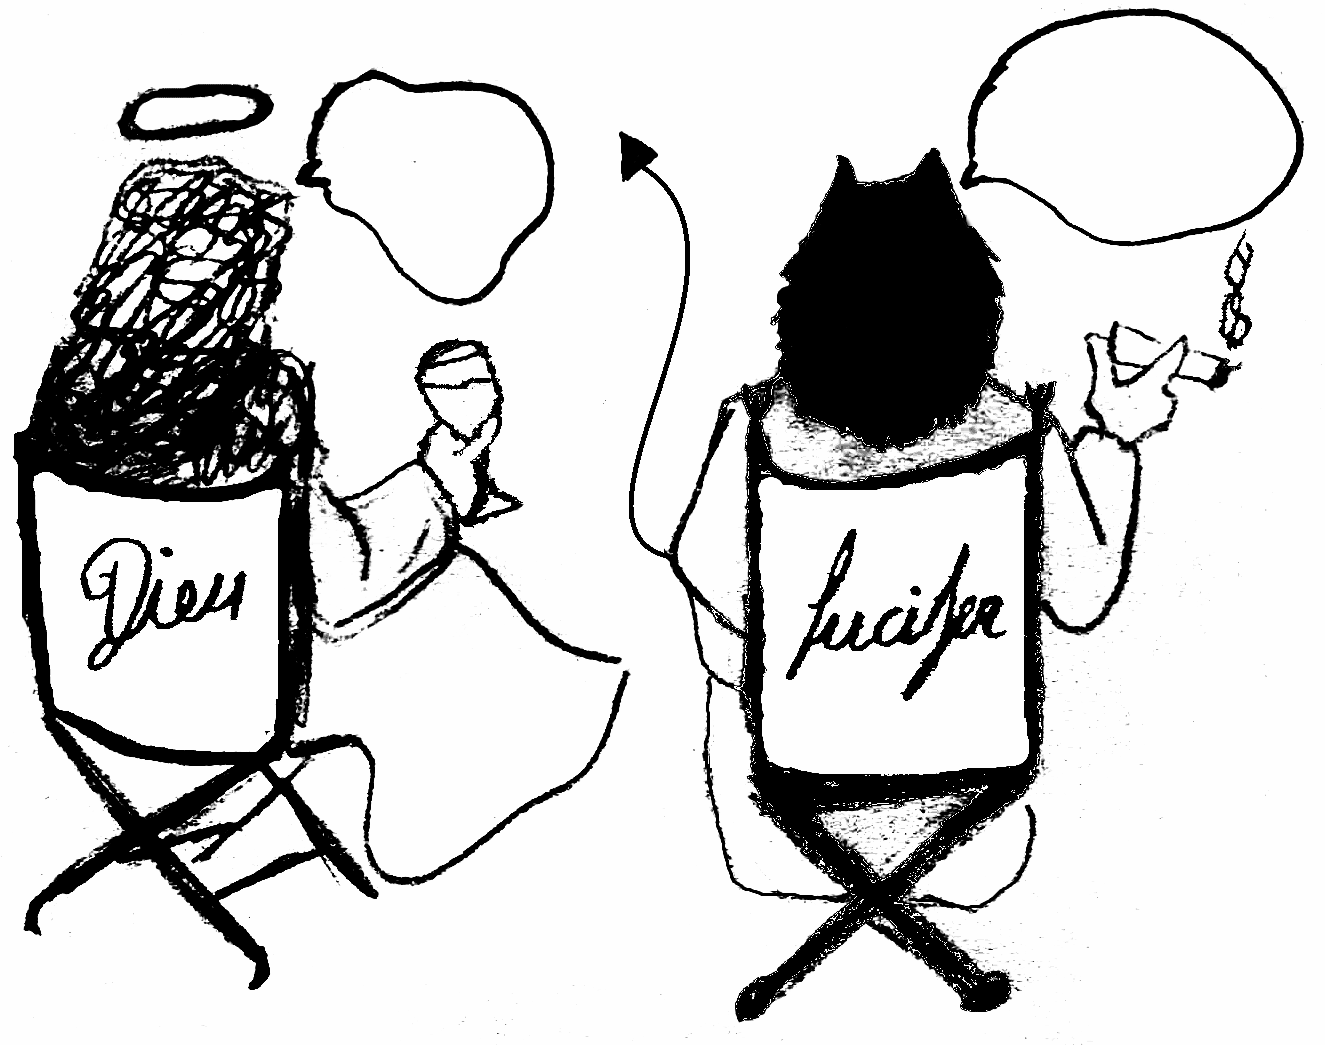
\includegraphics[width=0.5\textwidth]{images/amis_buvons.png}
 \end{figure}

\breakpage